\chapter{Transformações Lineares}

\section{Introdução}
Considere uma matriz $A\in {\mathbb{R}}^{m\times n}$. Quando efetuamos um produto entre uma matriz $A$ e um vetor $x$, estamos levando o espaço ${\mathbb{R}}^n$ no espaço ${\mathbb{R}}^m$:
\begin{align*}
    A : & \; {\mathbb{R}}^n \rightarrow {\mathbb{R}}^m\\
        & \; x \mapsto Ax=b
\end{align*}
Portanto, podemos encarar uma matriz como uma transformação no espaço.
\begin{center}
   	\begin{minipage}{0.5\textwidth}
	    \begin{exemplo}
		    \begin{equation*}
       		A=
       		\begin{pmatrix}
          	c & 0\\
          	0 & c
       		\end{pmatrix}
    		\end{equation*}
    		Esta transformação (às vezes chamada de \emph{homotetia}) não movimenta um vetor no plano, mas altera seu tamanho. Se $c\in {\mathbb{R}}$, e $v=(x,y)$, $Av = (cx,cy)$ está sobre a reta que passa pelo vetor $v$.
        \end{exemplo}
    \end{minipage}
    \begin{minipage}{0.4\textwidth}
    	\begin{center}
        	\begin{tikzpicture}[axis/.style={thick, ->, >=stealth'}]
            	\draw[axis] (0,0) -- (2,0);
                \draw[axis] (0,0) -- (0,2);
                \draw[thick, ->, >=stealth'] (0,0) -- (1,0.5);
                \draw[dashed] (-1,-0.5) -- (3,1.5);
                \node[anchor=west] at (2,0) {$x$};
                \node[anchor=west] at (0,2) {$y$};
                \node[anchor=west] at (1,0.4) {$v$};
            \end{tikzpicture}
        \end{center}
    \end{minipage}
\end{center}

\begin{center}
   	\begin{minipage}{0.5\textwidth}
		\begin{exemplo}
    		\begin{equation*}
        		A=
        		\begin{pmatrix}
           		0 &-1\\
           		1 & 0
        		\end{pmatrix}
    		\end{equation*}
    		Esta matriz rotaciona qualquer vetor por 90 graus no sentido anti-horário: $A(1,0) = (0,1)$, $A(0,1)=(-1,0)$.
		\end{exemplo}
    \end{minipage}
    \begin{minipage}{0.4\textwidth}
    	\begin{center}
        	\begin{tikzpicture}[axis/.style={thick, ->, >=stealth'}]
            	\draw[axis] (0,0) -- (2,0);
                \draw[axis] (0,0) -- (0,2);
                \draw[very thick, ->, >=stealth'] (0,0) -- (1.5,0.75);
                \node[anchor=west] at (2,0) {$x$};
                \node[anchor=west] at (0,2) {$y$};
                \node[anchor=west] at (1.5,0.6) {$v$};
                \draw[very thick, ->, >=stealth'] (0,0) -- (-0.75,1.5);
                \node[anchor=west] at (-0.8,1.6) {$Av$};
            \end{tikzpicture}
        \end{center}
    \end{minipage}
\end{center}

\begin{center}
   	\begin{minipage}{0.5\textwidth}
		\begin{exemplo}
    		\begin{equation*}
        		A = 
        		\begin{pmatrix}
           		0 &1\\
           		1 & 0
        		\end{pmatrix}
    		\end{equation*}
    		Esta matriz reflete todo vetor no eixo de simetria de 45 graus. 
		\end{exemplo}
    \end{minipage}
    \begin{minipage}{0.4\textwidth}
    	\begin{center}
        	\begin{tikzpicture}[axis/.style={thick, ->, >=stealth'}]
            	\draw[axis] (0,0) -- (2,0);
                \draw[axis] (0,0) -- (0,2);
                \draw[dashed] (-1,-1) -- (2,2);
                \draw[very thick, ->, >=stealth'] (0,0) -- (1.5,0.75);
                \node[anchor=west] at (2,0) {$x$};
                \node[anchor=west] at (0,2) {$y$};
                \node[anchor=west] at (1.5,0.6) {$v$};
                \draw[very thick, ->, >=stealth'] (0,0) -- (0.75,1.5);
                \node[anchor=west] at (0.8,1.6) {$Av$};
            \end{tikzpicture}
        \end{center}
    \end{minipage}
\end{center}

\begin{center}
   	\begin{minipage}{0.5\textwidth}
		\begin{exemplo}
    		\begin{equation*}
        		A =
        		\begin{pmatrix}
           		1 & 0\\
           		0 &0
        		\end{pmatrix}
    		\end{equation*}
    		Esta matriz toma qualquer vetor do espaço e projeta no subespaço definido por $x_2=0$, ou seja, no eixo $x_1$. Este eixo é o espaço coluna de $A$, enquanto que seu espaço nulo é o eixo $x_1=0$. 
		\end{exemplo}
    \end{minipage}
    \begin{minipage}{0.4\textwidth}
    	\begin{center}
        	\begin{tikzpicture}[axis/.style={thick, ->, >=stealth'}]
            	\draw[axis] (0,0) -- (2,0);
                \draw[axis] (0,0) -- (0,2);
                \draw[very thick, ->, >=stealth'] (0,0) -- (1.5,1.5);
                \node[anchor=west] at (2,0) {$x$};
                \node[anchor=west] at (0,2) {$y$};
                \node[anchor=west] at (1.5,1.5) {$v$};
                \draw[very thick, ->, >=stealth'] (0,0) -- (1.5,0);
                \node[anchor=west] at (1.3,-0.3) {$Av$};
                \draw[dashed] (1.5,1.5) -- (1.5,0);
            \end{tikzpicture}
        \end{center}
    \end{minipage}
\end{center}

É importante notar, no entanto, que algumas transformações não podem ser realizadas através de matrizes:

\begin{itemize}
    \item[(i)] É impossível mover a origem, já que $A0=0$.
    \item[(ii)] Se $Ax=x'$, então $A(2x) = 2x'$, ou seja, $A(cx)=cAx$.
    \item[(iii)] Se $Ax=x'$ e $Ay=y'$, então $A(x+y)=x'+y'$, ou seja, $A(x+y)=Ax+Ay$.
\end{itemize}

Estas regras vem da definição da multiplicação entre matrizes, e definem o que chamamos de \emph{transformação linear}.

\begin{defi}
Sejam $E,F$ espaços vetoriais sobre um mesmo corpo ${\mathbb{K}}$. Uma transformação linear $T$ é uma função $T:E\to F$ que associa a cada $u\in E$ um vetor $v=T(u) \in F$ e que satisfaz a condição seguinte: para todos $u,w\in E$ e $\alpha \in {\mathbb{K}}$ temos que
\begin{equation*}
	T(\alpha u+w) = \alpha T(u)+T(w).
\end{equation*}
\end{defi}

Para todo número $c,d\in {\mathbb{R}}$ e vetores $x,y\in {\mathbb{R}}^n$, a multiplicação de matrizes satisfaz a regra da linearidade
\begin{equation*}
    A(cx+dy)=c(Ax)+d(Ay).
\end{equation*}
Toda transformação que satisfaz esta propriedade é uma transformação linear. Portanto, toda matriz define uma transformação linear. Mas, será que toda transformação linear leva a uma matriz? Veremos que, em espaços de dimensão finita, isso é verdadeiro.

Tome como exemplo o espaço ${\mathcal{P}}_n$, polinômios de grau $\leq n$. Este espaço tem dimensão $n+1$.
\begin{exemplo}
    A diferenciação, $d/dx$, é uma transformação linear:
    \begin{align*}
        Ap &= \frac{d}{dx} p(x) \\
        &= \frac{d}{dx} (a_0+a_1x+\ldots+a_nx^n)\\
        & = a_1+2a_2x+\ldots+na_nx^{n-1}.
    \end{align*}
\end{exemplo}

\begin{exemplo}
    A integração de $0$ a $x$ também é linear (leva ${\mathcal{P}}_n$ a ${\mathcal{P}}_{n+1})$:
    \begin{align*}
        Ap &= \int_0^x p(x) dx \\
        &= \int_0^x (a_0+a_1x+\ldots+a_nx^n) dx \\
        &= a_0x + \ldots + \frac{a_n}{n+1} x^{n+1}.
    \end{align*}
\end{exemplo}

A definição abaixo nos dá uma ideia de onde essas transformações lineares vivem e das relações entre elas.

\begin{defi}
  Seja ${\mathcal{L}}(E;F)$ o conjunto das transformações lineares de $E$ em $F$. Então, ${\mathcal{L}}(E;F)$ é um espaço vetorial. As transformações lineares $T:E\rightarrow E$ são chamadas \emph{operadores lineares} em $E$. Por sua vez, as transformações lineares $\varphi:E\rightarrow {\mathbb{R}}$, com valores numéricos, são chamadas \emph{funcionais} lineares. Escreve-se $E^*$ em vez de ${\mathcal{L}}(E;{\mathbb{R}})$ e o conjunto $E^*$ dos funcionais lineares $\varphi:E\rightarrow {\mathbb{R}}$ chama-se \emph{espaço vetorial dual} de $E$.
\end{defi}

\section{Matriz de uma transformação linear}

A linearidade é importante pois nos dá uma propriedade crucial: se conhecermos a ação de uma transformação em todos os vetores da base, conhecemos a ação da transformação em todos os vetores do espaço gerado por esta base, visto que cada vetor do espaço é apenas combinação linear de todos os vetores da base. Depois que sabemos a ação de uma transformação na base, não há mais graus de liberdade possíveis: a transformação fica inteiramente determinada.

\begin{exemplo}
  Que transformação linear leva 
  \begin{align*}
    x_1 &= 
    \begin{pmatrix}
       1\\
       0
    \end{pmatrix}
    \text{ em } Ax_1 =
    \begin{pmatrix}
       2\\
       3\\
       4
    \end{pmatrix}
    \text{ e }\\
    x_2 &=
    \begin{pmatrix}
       0\\
       1
    \end{pmatrix}
    \text{ em } Ax_2 =
    \begin{pmatrix}
       4\\
       6\\
       8
    \end{pmatrix}
    ?
  \end{align*}
  A resposta deve ser a multiplicação pela matriz 
  \begin{equation*}
     A = \begin{pmatrix} 2 & 4\\ 3 & 6\\ 4 & 8 \end{pmatrix}.
  \end{equation*}
\end{exemplo}

Agora, considere outro problema: encontrar a matriz que representa a diferenciação, e a matriz que representa a integração em um intervalo. Basta, para isto, definirmos uma base para o espaço onde as transformações serão aplicadas. Para os polinômios de grau $\leq 3$, cuja dimensão é 4, existe uma base natural que é a base dos monômios,
\begin{equation*}
  p_1=1, \quad p_2=x, \quad p_3=x^2, \quad p_4=x^3.
\end{equation*}
Esta base não é única, mas é bastante conveniente. Agora, vamos olhar para o efeito da diferenciação nesta base: sejam $q_1 = 1$, $q_2 = x$, $q_3 = x^2$ em ${\mathcal{P}}_2$. Então
\begin{align*}
  Ap_1&=0, \quad Ap_2 = 1=q_1, \\ 
  Ap_3&=2x = 2q_2, \quad Ap_4 = 3x^2=3q_3.
\end{align*}
Note que 
\begin{equation*}
   A : {\mathcal{P}}_3 \rightarrow {\mathcal{P}}_2, \mbox{ tal que } A_{\text{diff}} =
      \begin{pmatrix}
         0 & 1 & 0 & 0\\
         0 & 0 & 2 & 0\\
         0 & 0 & 0 & 3
      \end{pmatrix}.
\end{equation*}
A derivada de qualquer outra combinação de polinômios é uma combinação linear dos membros da base, e portanto aplicar a matriz da transformação a este polinômio é equivalente a aplicá-la aos vetores da base e combinar os resultados.

Suponha que os vetores $p_1,\ldots,p_n$ são base para o espaço $V$, e $q_1,\ldots,q_m$ formam uma base para o espaço $W$. Então, cada transformação linear $A$ de $V$ para $W$ é representada por uma matriz. A $j$-ésima coluna é encontrada ao aplicarmos $A$ ao $j$-ésimo vetor da base de $W$; o resultado $Ap_j$ é combinação dos $q$ e os coeficientes desta combinação vão na coluna $j$ de $A$:
\begin{equation*}
  Ap_j = a_{1,j}q_1+\ldots+a_{m,j}q_m.
\end{equation*}
Para a matriz de diferenciação, a coluna 1 veio de $p_1$: sua derivada era zero, então a primeira coluna era nula. A última coluna veio de $x^3$: a derivada era $3x^2$, e assim o coeficiente 3 está na linha correspondente a $x^2=p_3$.

Fazendo a mesma coisa para a integração, que vai do espaço ${\mathcal{P}}_2$ no espaço ${\mathcal{P}}_3$. Devemos então escolher uma base para ${\mathcal{P}}_3$. A base mais natural para este espaço é justamente $q_1=1, q_2=x, q_3=x^2,q_4 = x^3$. Desta forma, teremos, para cada vetor da base do espaço ${\mathcal{P}}_3$:
\begin{align*}
  Ap_1&=x=q_2, \quad Ap_2=\frac{1}{2}x^2=\frac{1}{2}q_3, \\
  Ap_3&=\frac{1}{3}x^3=\frac{1}{3}q_4.
\end{align*}
Assim, a matriz que representa esta transformação linear é 
\begin{equation*}
  A_{\text{int}} =
  \begin{pmatrix}
     0 & 0 & 0\\
     1 & 0 & 0\\
     0 & \frac{1}{2}& 0 \\
     0 & 0 & \frac{1}{3}\\
  \end{pmatrix}.
\end{equation*}

{\bf Observação:} Enxergamos a integração como a operação inversa da diferenciação, isto é, a integração seguida da diferenciação nos dão o resultado original de volta. Se tomarmos a matriz de diferenciação na base das cúbicas, que é uma matriz $3\times 4$, teremos:
\begin{equation*}
  A_{\text{diff}}=
  \begin{pmatrix}
     0 & 1 & 0 & 0\\
     0 & 0 & 2 & 0\\
     0 & 0 & 0 & 3
  \end{pmatrix}
  , \text{ e } A_{\text{diff}} A_{\text{int}} =
  \begin{pmatrix}
     1& & \\
     &1& \\
     & &1
  \end{pmatrix}.
\end{equation*}
Portanto, o operador de diferenciação nesta base é a inversa à esquerda da integração. Como para matrizes retangulares é impossível termos inversas dos dois lados, o produto $A_{\text{int}}A_{\text{diff}}$ não pode ser igual à identidade; mas isto não ocorre de qualquer forma, já que a derivada de uma constante é zero, e a integral de zero nunca pode trazer esta constante de volta (a primeira linha do produto citado é nula).

As transformações lineares aqui representadas (e todas as outras) tem representação matricial, mas uma transformação linear não é uma matriz: uma matriz representa a transformação em uma base dada. Portanto, a matriz usada para representarmos uma transformação linear varia de acordo com a base escolhida para o espaço.

\subsection{Matriz de uma transformação linear em relação a uma base do domínio e a uma base do contradomínio.}

Uma transformação linear $T:E\rightarrow F$ é uma função especial que é linear, e vai do espaço vetorial $E$ no espaço vetorial $F$. Em geral, para definirmos uma função, precisamos definir o valor de $f(x)$ para todo $x$ no domínio de $f$. No caso das transformações lineares, é bem mais fácil definirmos esta função, pois basta fazê-lo em cada elemento da base.

Sejam $E,F$ espaços vetoriais de dimensão finita e $\beta=\{u_1,\dots,u_n\}$ uma base de $E$. Todo vetor $v\in E$ se exprime, de modo único, como combinação linear
\begin{equation*}
  v=x_1u_1+\ldots+x_nu_n
\end{equation*}
de elementos da base $\beta$. Para qualquer transformação linear $T:E\rightarrow F$ e para qualquer vetor $v\in E$, temos que 
\begin{align*}
  T(v) &= T(x_1u_1+\ldots+x_nu_n)\\
  &= x_1 T(u_1) + \ldots + x_nT(u_n),
\end{align*}
ou seja, a definição de $T$ depende apenas da aplicação da transformação linear nos vetores $u_i\in \beta$. 

Como consequência, se quisermos definir uma transformação linear $T:E \to F$, basta escolhermos uma base $\gamma$ para $F$, e para cada $j=1,\ldots,n$ um vetor 
\begin{equation*}
  v_j=(a_{1j},a_{2j},\ldots,a_{mj})_{\gamma} \in F
\end{equation*}
e dizer que $v_j = T(u_j)$ é a imagem do $j$-ésimo vetor da base $\beta$ pela transformação linear $T$. A partir daí, fica determinada a imagem $T(v)$ de qualquer vetor $v\in E$, pois se 
\begin{equation*}
  v=x_1u_1+\ldots+x_nu_n = (x_1,\ldots,x_n)_{\beta},
\end{equation*}
então
\begin{align*}
    y &= T(v) = T\left(\sum_{j=1}^n x_ju_j\right)\\
    &= \sum_{j=1}^n x_jT(u_j) \\
    &= \sum_{j=1}^n \left( a_{1j}x_j,a_{2j}x_j,\ldots,a_{mj}x_j\right)_{\gamma} \\
    &= \left( \sum_{j=1}^n a_{1j}x_j,\sum a_{2j}x_j,\ldots,\sum a_{mj}x_j \right)_{\gamma},
\end{align*}
ou seja, cada coordenada $y_i$ do vetor $y$ na base $\gamma$ é calculada como
\begin{align*}
    y_1 &= a_{11}x_1 + a_{12}x_2 + \ldots + a_{1n}x_n\\
    y_2 &= a_{21}x_1 + a_{22}x_2 + \ldots + a_{2n}x_n\\
        & \vdots  \\
    y_m &= a_{m1}x_1 + a_{m2}x_2 + \ldots + a_{mn}x_n
\end{align*}
Portanto, toda transformação linear $T:E \to F$ fica inteiramente determinada por uma matriz $A\in {\mathbb{K}}^{m\times n}$. Os vetores-coluna desta matriz são as coordenadas dos vetores $v_j$ na base $\gamma$, em que cada $v_j=T(u_j)$, ou seja, imagem do vetor $u_j$ da base $\beta$ de $E$. A imagem de $T(v)$ é o vetor $(y_1,\ldots,y_m)_{\gamma}\in F$ cujas coordenadas são dadas pelas equações acima.

O resultado a seguir será útil mais à frente.

\begin{teo}
  Para toda matriz $A\in {\cal{M}}(m\times n)$, o número de linhas l.i. de $A$ é igual ao número de colunas l.i. de $A$.
\end{teo}

\begin{proof}
Seja $p$ o número de colunas l.i. da matriz $A$. Então existem $p$ vetores 
\begin{equation*}
   w_k =\begin{pmatrix} w_{1k}\\\vdots\\w_{mk}\end{pmatrix} \in {\mathbb{R}}^m
\end{equation*}
 tais que cada uma das colunas 
\begin{equation*}
   a_{(:,j)}=\begin{pmatrix}a_{1j}\\\vdots\\a_{mj}\end{pmatrix}, 1\leq j \leq n
\end{equation*}
de $A$ é combinação linear dos $w_1,\ldots,w_p$:
\begin{equation*}
   a_{(:,j)} = \sum_{k=1}^p c_{kj}w_k, \qquad 1\leq j \leq n.
\end{equation*}
Tomando a $i$-ésima coordenada de cada um dos membros desta equação, vemos que
\begin{equation}\label{eq:duas}
   a_{ij} = \sum_{k=1}^p c_{kj}w_{ik}=\sum_{k=1}^p w_{ik}c_{kj},
\end{equation}
para quaisquer $i$, $j$, com $1\leq i \leq m$ e $1\leq j \leq n$. Considerando agora os vetores-linha $a_{(i,:)}=(a_{i1},\ldots,a_{in})$ da matriz $A$, juntamente com os vetores $c_k=(c_{k1},\ldots,c_{kn})$, $1\leq k\leq p$, observamos que a igualdade entre o primeiro e o terceiro membros de \eqref{eq:duas} significa que, para todo $i=1,\ldots,m$ tem-se 
\begin{equation*}
   a_{(i,:)} = \sum_{k=1}^p w_{ik} c_k, \qquad 1\leq i \leq m.
\end{equation*}
Assim, os vetores linha de $A$ são combinações lineares de $c_1,\ldots,c_p$, portanto o número de linhas l.i. de $A$ é $\leq p$. Aplicando este resultado à matriz $A^T$, que tem como linhas as colunas de $A$, concluimos que o o número de colunas l.i. de $A$ é menor ou igual ao número de linhas l.i. de $A$ e assim temos o resultado completo.
\end{proof}

\section{Rotações, projeções e reflexões.}

Já vimos que rotações de 90 graus, projeções no eixo $x$ e reflexões com relação à linha de 45 graus em ${\mathbb{R}}^2$ eram representadas por matrizes simples da forma
\begin{equation*}
  Q=
  \begin{pmatrix}
     0 & -1\\
     1 & 0
  \end{pmatrix}
  , \qquad P=
  \begin{pmatrix}
     1 & 0\\
     0 & 0
  \end{pmatrix}
  , \qquad H=
  \begin{pmatrix}
     0 & 1\\
     1 & 0
  \end{pmatrix}
\end{equation*}
respectivamente. Mas é lógico pensar que rotações com outros ângulos, reflexões e projeções em outros eixos serão igualmente simples, já que estas são todas transformações lineares que passam pela origem ($A0=0$). Assim, vamos primeiramente considerar o plano e seus vetores básicos $(1,0), (0,1)$ para tentarmos visualizar estas transformações em geral.

\paragraph*{Rotação.} Na Figura~\ref{fig:rotacao}, mostramos a rotação por um ângulo $\theta$ no sentido anti-horário. Podemos ver o efeito desta rotação nos dois vetores básicos, onde $c=\cos{\theta}$ e $s=\sin{\theta}$. A rotação aplicada ao primeiro vetor da base resulta em $(\cos{\theta}, \sin{\theta})$, cujo comprimento é ainda 1. Se aplicada ao segundo vetor, a rotação resulta em $(-\sin{\theta},\cos{\theta})$. Assim, pela definição da transformação linear que vimos antes, estas são as colunas da matriz da transformação, e assim temos $Q_\theta$.
\begin{figure}[!h]
   \begin{center}
   \begin{tikzpicture}[axis/.style={thick, ->, >=stealth'}, >=stealth']
      \draw[axis] (-0.5,0) -- (2,0);
      \draw[axis] (0,-0.5) -- (0,2);
      \draw[very thick, ->] (0,0) -- (1,0);
      \node[anchor=west] at (1,-0.3) {$(1,0)$};
      \draw[very thick, ->] (0,0) -- (0,1);
      \node[anchor=east] at (0,1) {$(0,1)$};
      % Seta (-sin(theta),cos(theta))
      \draw[thick,->] (0,0) -- (-0.86,0.5);
      \node[anchor=east] at (-0.86,0.5) {$(-s,c)$};
      % Seta (cos(theta),sin(theta))
      \node[anchor=west] at (0.5,0.86) {$(c,s)$};
      \draw[thick, ->] (0,0) -- (0.5,0.86);
      % Arcos
      \draw[->] (0.5,0) arc (0:60:0.5cm);
	  \node[font=\scriptsize, anchor=south] at (-0.3,0.4) {$\theta$};
      \draw[->] (0,0.5) arc (90:150:0.5cm);
      \node[font=\scriptsize, anchor=west] at (0.4,0.3) {$\theta$};
   \end{tikzpicture}
   \caption{Rotação por um ângulo $\theta$.}
   \label{fig:rotacao}
   \end{center}
\end{figure}
Com esta transformação, podemos exemplificar o comportamento das transformações enquanto matrizes.
\begin{itemize}
\item[(i)] A inversa de $Q_\theta$ equivale à rotação por $\theta$ no sentido contrário:
  \begin{equation*}
    Q_\theta Q_{-\theta} = 
    \begin{pmatrix}
       c&-s\\ 
       s&c
    \end{pmatrix}
    \begin{pmatrix}
       c&s\\
       -s & c
    \end{pmatrix}
    =
    \begin{pmatrix}
       1 & 0\\
       0 & 1
    \end{pmatrix}.
  \end{equation*}
  \item[(ii)] O quadrado de $Q_\theta$ (ou seja, a aplicação desta matriz duas vezes sobre o mesmo vetor) equivale à rotação por um ângulo $2\theta$:
    \begin{align*}
      Q_{\theta}^2 &= 
      \begin{pmatrix}
         c & -s\\
         s & c
      \end{pmatrix}
      \begin{pmatrix}
         c & -s\\
         s & c
      \end{pmatrix}
      \\
      & = 
      \begin{pmatrix}
         c^2-s^2 & -2cs\\
         2cs & c^2-s^2
      \end{pmatrix}
      \\
      & = 
      \begin{pmatrix}
         \cos{2\theta} & -\sin{2\theta}\\
         \sin{2\theta} & \cos{2\theta}
      \end{pmatrix}.
    \end{align*}
  \item[(iii)] O produto de $Q_\theta$ e $Q_\varphi$ é equivalente à rotação por $\theta+\varphi$:
  \begin{align*}
     Q_{\theta}Q_\varphi &=
     \begin{pmatrix}
        \cos{\theta} & -\sin{\theta}\\
        \sin{\theta} & \cos{\theta}
     \end{pmatrix}
     \begin{pmatrix}
        \cos{\varphi} & -\sin{\varphi}\\
        \sin{\varphi} & \cos{\varphi}
     \end{pmatrix}
     \\
     &=
     \begin{pmatrix}
        \cos{\theta}\cos{\varphi}-\sin{\theta}\sin{\varphi} & -\cos{\theta}\sin{\varphi}-\sin{\theta}\cos{\varphi}\\
        \cos{\theta}\sin{\varphi}+\sin{\theta}\cos{\varphi} & -\sin{\theta}\sin{\varphi} + \cos{\theta}\cos{\varphi}
     \end{pmatrix}
     \\
     &=
     \begin{pmatrix}
        \cos{(\theta+\varphi)} & -\sin{(\theta+\varphi)}\\
        \sin{(\theta+\varphi)} & \cos{(\theta+\varphi)}
     \end{pmatrix}
     = Q_{\theta+\varphi}.
  \end{align*}
\end{itemize}

Estas propriedades não acontecem por acidente: a multiplicação de matrizes é definida para que estas propriedades sejam verdadeiras para as transformações lineares: o produto das matrizes das transformações lineares é o produto das transformações, ou mais exatamente, a composição das transformações.

\paragraph*{Projeção} Na Figura~\ref{fig:projecao} representamos a projeção dos vetores básicos na reta determinada pelo ângulo $\theta$.
\begin{figure}[!h]
  \centering
  \begin{tikzpicture}[axis/.style={thick, ->, >=stealth'}, >=stealth']
     % Eixos
     \draw[axis] (0,-0.5) -- (0,3);
     \draw[axis] (-0.5,0) -- (3,0);
     \draw[very thick, ->] (0,0) -- (2,0);
     \node[anchor=north west] at (2,0) {$(1,0)$};
     \draw[very thick, ->] (0,0) -- (0,2);
     \node[anchor=west] at (0,2) {$(0,1)$};
     % Reta de ângulo theta
     \draw (0,0) -- (2.3,1.92);
     % Arco
     \draw[->] (0.5,0) arc (0:40:0.5cm);
     \node[font=\scriptsize] (t) at (0.8,0.3) {$\theta$};
     % Projeções
     \draw[densely dashed, very thick, ->] (2,0) -- (1.17,0.98);
     \draw[densely dashed, very thick, ->] (0,2) -- (0.98,0.82);
     % Anotacoes
     \node[anchor=west, font=\scriptsize] at (1.2,0.98) {$(sc,s^2)$};
     \node[anchor=east, font=\scriptsize] at (0.98,0.82) {$(c^2,sc)$};
  \end{tikzpicture}
  \caption{Projeção ortogonal na reta que faz ângulo $\theta$ com o eixo $x$.}
  \label{fig:projecao}
\end{figure}
Note que o comprimento da projeção é $c=\cos{\theta}$. Assim, o ponto de projeção de $(1,0)$ é exatamente $c(c,s)$. Similarmente, a projeção de $(0,1)$ é $s(c,s)$.

A matriz desta transformação não pode possuir inversa, pois a projeção não pode ser desfeita. Pontos do tipo $(-s,c)$ são projetados na origem (voltaremos a este fato mais tarde). Ao mesmo tempo, todos os pontos na linha $\theta$ são projetados neles mesmos! Em outras palavras, projetar duas vezes é o mesmo que projetar uma vez, e então $P^2=P$:
\begin{equation*}
  P^2=
  \begin{pmatrix}
     c^2 & cs\\
     cs & s^2
  \end{pmatrix}
  ^2 = 
  \begin{pmatrix}
     c^2(c^2+s^2) & cs(c^2+s^2)\\
     cs(c^2+s^2) & s^2(c^2+s^2)
  \end{pmatrix}.
\end{equation*}

\paragraph*{Reflexão} Na Figura \ref{fig:reflexao}, vemos a reflexão de $(1,0)$ na reta que faz ângulo $\theta$ com o eixo $x$. O comprimento da reflexão é igual ao comprimento do vetor original, assim como na rotação. No entanto, estas transformações são bem diferentes: aqui, a reta definida por $\theta$ continua a mesma, e os pontos são apenas refletidos, como que por um espelho. 
\begin{figure}[!h]
  \centering
  \begin{tikzpicture}[>=stealth',scale=1.5]
     % Eixos
     \draw (0,-0.5) -- (0,2.5);
     \draw (-0.5,0) -- (2.5,0);
     % Setas (2,0) e (0,2)
     \draw[very thick, ->] (0,0) -- (2,0);
     \node[anchor=west] at (2,-0.3) {$(1,0)$};
     % Reta de ângulo theta
     \draw (0,0) -- (2.3,1.92);
     % Arco
     \draw[->] (0.7,0) arc (0:50:0.5cm);
     \node at (0.8,0.3) {$\theta$};
     % Reflexão
     \draw[densely dashed, thick] (2,0) -- (0.4,2.0);
     \draw[very thick, ->] (0,0) -- (0.4,2);
     \node[anchor=west] at (0.4,2) {$H(1,0)$};
  \end{tikzpicture}
  \caption{Reflexão em torno do eixo que faz ângulo $\theta$ com o eixo $x$.}
  \label{fig:reflexao}
\end{figure}

A matriz desta transformação tem uma propriedade especial: $H^2=I$, ou seja, duas reflexões trazem de volta o original. Assim, uma reflexão é sua própria inversa. Para vermos isso em termos matriciais, note primeiramente que $H=2P-I$. Assim, $Hx+x=2Px$, ou seja, o elemento refletido mais o original é igual a duas vezes sua projeção. Portanto,
\begin{equation*}
  H^2 = (2P-I)^2 = 4P^2-4P+I=I,
\end{equation*}
já que toda projeção satisfaz $P^2=P$.

\section{Produto de transformações lineares}

\begin{defi}
Suponha que $T$ e $S$ são transformações lineares tais que
\begin{equation*}
  T: V\to W, \qquad S: U\to V.
\end{equation*}
Então,
\begin{align*}
  (T\circ S) :& U\to V\to W\\
      & u \mapsto S(u) \mapsto T(S(u)).
\end{align*}
Logo, a composição $(T\circ S):U\to W$ também é uma transformação linear.
\end{defi}

\paragraph*{Observação}
  Sejam $P,Q:{\mathbb{R}}^2 \rightarrow {\mathbb{R}}^2$ projeções ortogonais sobre duas retas do plano, uma das quais é perpendicular à outra. Todo vetor $v\in {\mathbb{R}}^2$ é a diagonal de um retângulo que tem $Pv$ e $Qv$ como lados. Segue-se então que $v = Pv+Qv$ para todo $v\in {\mathbb{R}}^2$, ou seja, $P+Q=I$. Logo, $Q=I-P$ e portanto $PQ=P(I-P)=P-P^2$. Como sabemos que a projeção satisfaz $P^2=P$, temos que $PQ=0$ mesmo com $P,Q\ne 0$. 

\begin{defi}
    Um operador $A$ chama-se \emph{nilpotente} quando, para algum $n\in {\mathbb{N}}$, tem-se $A^n=0$.
\end{defi}

\begin{exemplo}
    O operador de derivação que vimos anteriormente é nilpotente, pois se ele age de ${\mathcal{P}}_{n}$ em ${\mathcal{P}}_{n-1}$, então $D^{n+1}p=0$ para todo $p$, ou seja, $D^{n+1}=0$.
\end{exemplo}

\section{Os Espaços Fundamentais}

\subsection*{Imagem}

Agora, vamos considerar o exemplo de um sistema de equações lineares de três equações e duas incógnitas:
\begin{equation*}
   \begin{pmatrix}
      1 & 0\\
      5 & 4\\
      2 & 4
    \end{pmatrix}
    \begin{pmatrix}
      u\\
      v
    \end{pmatrix}
    =
    \begin{pmatrix}
      b_1\\
      b_2\\
      b_3
    \end{pmatrix}.
\end{equation*}

Como nesse caso temos mais equações que incógnitas, é bastante provável que o sistema não tenha solução. Um sistema com $m>n$ poderá ser resolvido se o lado direito do sistema (aqui, $b$) estiver contido em um subespaço vetorial especial: \emph{o sistema $Ax=b$ poderá ser resolvido se e somente se o vetor $b$ puder ser escrito como combinação linear das colunas de $A$.} 

Para ver isto, note que o sistema pode ser reescrito da seguinte forma:
\begin{equation*}
  u \begin{pmatrix}
      1\\
      5\\
      2
    \end{pmatrix}
   + v
    \begin{pmatrix}
      0\\
      4\\
      4
    \end{pmatrix}
    = 
    \begin{pmatrix}
      b_1\\
      b_2\\
      b_3
    \end{pmatrix}.
\end{equation*}

Assim, note que o subconjunto dos vetores que podem ser gerados como lado direito do sistema é exatamente o conjunto de todas as combinações lineares das colunas de $A$. Portanto, $Ax=b$ pode ser resolvido se e somente se $b$ estiver contido no plano que é gerado pelos dois vetores coluna de $A$. Se $b$ não estiver contido neste plano, então ele não pode ser obtido como combinação linear das colunas de $b$. Neste caso, o sistema não tem solução.

Se $A$ representa uma transformação linear, este plano definido pelas colunas de $A$, é um subespaço importante chamado \emph{espaço coluna de $A$}, ou \emph{imagem} de $A$ (ou ainda, imagem da transformação representada pela matriz $A$). Por um lado, se $A=0$ então o espaço coluna de $A$ será formado apenas pelo vetor $b=0$; no outro extremo, qualquer matriz inversível em ${\mathbb{R}}^{n\times n}$ terá todo o espaço ${\mathbb{R}}^n$ como espaço coluna (qualquer lado direito em ${\mathbb{R}}^n$ define uma solução para o sistema).

\begin{defi}
	Seja $T:E\to F$ uma transformação linear definida entre espaços vetoriais $E,F$ sobre um mesmo corpo ${\mathbb{K}}$. Então a \emph{imagem} de $T$ é um subespaço vetorial definido como
    \begin{equation*}
	    {\mathcal{I}}m(T) = \{ y \in F \,|\, y=T(x), \text{ para algum } x\in E\}.
    \end{equation*}
\end{defi}

Verificamos se esse subconjunto é realmente um subespaço:

\begin{itemize}
\item[(i)] Suponha que $y_1, y_2\in {\mathcal{I}}m(T)$. Então, existem $x_1, x_2 \in E$ tais que $T(x_1)=y_1$ e $T(x_2) = y_2$. Logo, podemos escrever 
  \begin{equation*}
    y_1 + y_2 = T(x_1) + T(x_2) = T(x_1+x_2),
  \end{equation*}
  onde a última igualdade é válida pois $T$ é linear. Assim, $y_1+y_2$ pode ser escrito como $T(w)$, com $w = x_1+x_2 \in E$ (pois $E$ é espaço vetorial), e assim também pertence à imagem de $T$.
\item[(ii)] Seja $\alpha \in {\mathbb{K}}$ e $y \in {\mathcal{I}}m(T)$. Então, $\alpha y = \alpha T(x)$ para algum $x\in E$. Isto implica que $\alpha y = T(\alpha x)$, (já que $T$ é linear) e portanto, $\alpha y$ também pertence à imagem de $T$.
\end{itemize}

Portanto, a imagem é, de fato, um subespaço linear. 

\begin{defi}
	Seja $T:E\to F$ uma transformação linear como acima. Então chamamos a dimensão da imagem de $T$ de \emph{posto} de $T$ (ou \emph{rank} de $T$).
\end{defi}

Se a transformação linear $T$ tem representação como uma matriz $A$ com relação a uma base de $E$ e uma base de $F$, então podemos falar da imagem de $A$ como sendo 
\begin{equation*}
	{\mathcal{I}}m(A) = \{ b\in F : b=Ax, \text{ para algum } x \in E\}.
\end{equation*}
Isso significa que $b$ está na imagem de $A$ se e somente se o sistema $Ax=b$ tem solução. Neste caso, podemos escrever
\begin{align*}
	b &= Ax\\
      &= A(:,1)x_1 + A(:,2)x_2 + \ldots + A(:,n)x_n,
\end{align*}
em que $A(:,j)$ representa a coluna $j$ de $A$. Desta forma, $b \in {\mathcal{I}}m(A)$ se e somente se $b$ pode ser escrito como combinação linear das colunas de $A$ (em que os coeficientes da combinação linear são as entradas de $x$). Com isso, o posto da matriz $A$ é igual ao número de colunas l.i. de $A$ (que é igual ao número de linhas l.i. de $A$ por um teorema anterior).

Como encontrar uma base para a imagem de uma matriz $A$? Se a matriz $U$ é a matriz na forma escada obtida depois de aplicarmos a $A$ as operações elementares da eliminação gaussiana, então a imagem de $A$ é diferente da imagem de $U$, mas estes dois espaços têm a mesma dimensão. Para vermos isso, basta observarmos que o número de colunas l.i. de $U$ sempre será igual ao número de colunas l.i. de $A$, visto que os pivôs aparecem em $U$ justamente nas colunas que eram l.i. em $A$. 

Para recuperarmos uma base para a imagem de $A$, basta realizarmos a eliminação para obtermos $U$; os índices das colunas de $U$ que formam uma base para a sua imagem (as colunas que tem os pivôs da eliminação) correspondem aos índices das colunas de $A$ que são base para sua imagem. Isto acontece pois o sistema homogêneo $Ax=0$ equivale ao sistema homogêneo $Ux=0$; portanto, $Ax=0$ determina, assim como $Ux=0$, a dependência entre os vetores coluna da matriz $A$ (e de $U$), com coeficientes $x$, idênticos aos dois sistemas. Se um conjunto de colunas de $A$ é l.i., então as colunas correspondentes de $U$ também são l.i.

\begin{exemplo}
Finalmente, chegamos ao caso mais fácil, em que o posto é o menor possível (exceto pela matriz nula que possui posto 0). 
\begin{exemplo}
   \begin{equation*}
      A=
      \begin{pmatrix}
         2 & 1 & 1\\
         4 & 2 & 2\\
         8 & 4& 4\\
         -2 & -1 & -1
      \end{pmatrix}.
   \end{equation*}
   Cada linha é um múltiplo da primeira, e assim o espaço gerado pelas linhas de $A$ é unidimensional. De fato, podemos escrever esta matriz como um produto entre um vetor linha e um vetor coluna:
   \begin{equation*}
      A=
      \begin{pmatrix}
         2 & 1 & 1\\
         4 & 2 & 2\\
         8 & 4& 4\\
         -2 & -1 & -1
      \end{pmatrix}
      =
      \begin{pmatrix}
         1\\
         2\\
         4\\
         -1
      \end{pmatrix}
      \begin{pmatrix}
         2 &  1 &  1
      \end{pmatrix}.
   \end{equation*}
\end{exemplo}
Ao mesmo tempo, as colunas também são múltiplos do mesmo vetor coluna, e assim o espaço gerado pelas colunas também tem dimensão 1.
\end{exemplo}

\begin{teo}
	Toda matriz de posto 1 pode ser escrita como $A=uv^T$.
\end{teo}

\subsection*{Núcleo}

Agora, queremos analisar as possíveis soluções de um sistema $Ax=0$. Obviamente, a solução $x=0$ sempre é possível, mas podem haver outros $x\in {\mathbb{R}}^n$ que satisfaçam $Ax=0$, inclusive infinitas soluções deste tipo (isto sempre acontece quando temos mais variáveis do que equações, ou seja, $n>m$ - Teorema anterior). O conjunto das soluções do sistema homogêneo $Ax=0$ é também um subespaço vetorial.

\begin{defi}
	Seja $T:E\to F$ uma transformação linear. Então o \emph{núcleo} de $T$ (ou \emph{espaço nulo}, ou \emph{kernel} de $T$) é o subespaço vetorial definido como
    \begin{equation*}
    	{\mathcal{N}}(T) = \{ x \in E \, | \, T(x)=0 \}.
    \end{equation*}
\end{defi}

Analogamente ao caso da imagem, podemos calcular o núcleo da matriz que representa uma transformação linear encontrando todas as soluções do sistema homogêneo definido por essa matriz.

É fácil encontrarmos o núcleo para a matriz do exemplo anterior: basta tomarmos 
\begin{equation*}
   \begin{pmatrix}
      1 & 0\\
      5 & 4\\
      2 & 4
    \end{pmatrix}
    \begin{pmatrix}
      u\\
      v
    \end{pmatrix}
    = 
    \begin{pmatrix}
      0\\
      0\\
      0
    \end{pmatrix}
\end{equation*}
para percebermos que, da primeira equação, temos que $u=0$, e pela segunda equação devemos ter igualmente $v=0$. Portanto, neste caso, apenas o vetor nulo faz parte do núcleo da matriz.

Vamos supor agora que a matriz do sistema é
\begin{equation*}
  B = 
    \begin{pmatrix}
      1 & 0 & 1\\
      5 & 4 & 9\\
      2 & 4 & 6
    \end{pmatrix}.
\end{equation*}
A imagem desta matriz é igual à imagem de $A$, já que a terceira coluna é combinação linear das outras duas. No entanto, o núcleo desta matriz contém qualquer múltiplo do vetor $(1,1,-1)$. Portanto, este subespaço é uma reta que passa pela origem.


\section{Sistemas Retangulares}

Considere a seguinte matriz.
\begin{equation*}
  A = 
    \begin{pmatrix}
      1 & 3 & 3 & 2\\
      2 & 6 & 9 & 5\\
      -1 & -3 & 3 & 0
    \end{pmatrix}
\end{equation*}
O primeiro pivô é $a_{11} \ne 0$, e assim teremos
\begin{equation*}
  A \rightarrow 
    \begin{pmatrix}
      1 & 3 & 3 & 2\\
      0 & 0 & 3 & 1\\
      0 & 0 & 6 & 2
    \end{pmatrix}
\end{equation*}
O candidato a segundo pivô é zero, e assim vamos procurar embaixo dele por uma entrada não-nula. No entanto, todas as entradas abaixo dele são também nulas, e assim poderíamos parar a eliminação por aqui. Mas como esta matriz é retangular, não precisamos declarar a matriz singular; podemos apenas continuar com a eliminação na próxima coluna. Assim, teremos
\begin{equation*}
  U = 
    \begin{pmatrix}
      1 & 3 & 3 & 2\\
      0 & 0 & 3 & 1\\
      0 & 0 & 0 & 0
    \end{pmatrix}
\end{equation*}
pois na quarta coluna o candidato a pivô é nulo, e não podemos fazer mais nenhuma operação.

Assim, podemos como nas matrizes quadradas decompor $A = LU$; neste caso $L = \begin{pmatrix}
    1 & 0 & 0\\
    2 & 1 & 0\\
    -1 & 2 & 1
  \end{pmatrix}$. Podemos notar assim que $L$ é uma matriz $3\times 3$, ou seja, quadrada de dimensão igual ao número de linhas das matrizes $A$ e $U$. Caso seja necessário trocar uma linha pela outra no processo e eliminação para evitarmos um pivô nulo, podemos encontrar uma matriz de permutação $P$ tal que $PA=LU$. Resumimos tudo isso no seguinte resultado.

A qualquer matriz $A\in {\mathbb{R}}^{m\times n}$ correspondem uma matriz de permutação $P$, uma matriz triangular inferior $L$ com diagonal unitária, e uma matriz $m\times n$ na forma escada $U$ tais que $PA=LU$.

Nosso objetivo no momento é olhar para esta forma final e verificar quais as possibilidades para o sistema $Ax=b$.

Se $b=0$, então as operações da eliminação não tem efeito algum no vetor $b$; portanto as soluções de $Ax=b$ são as mesmas de $Ux=0$:
\begin{equation*}
  Ux =
    \begin{pmatrix}
      1 & 3 & 3 & 2\\
      0 & 0 & 3 & 1\\
      0 & 0 & 0 & 0 
    \end{pmatrix}
    \begin{pmatrix}
      x_1\\
      x_2\\
      x_3\\
      x_4
    \end{pmatrix}
    =
    \begin{pmatrix}
       0\\
       0\\
       0
    \end{pmatrix}.
\end{equation*}
As variáveis $x_1,x_2,x_3$ e $x_4$ podem ser concentradas em dois grupos: as variáveis básicas, que correspondem a colunas com pivôs não-nulos (neste caso, $x_1$ e $x_3$) e as variáveis livres, correspondentes a colunas sem pivôs (neste caso $x_2$ e $x_4$).

Para encontrarmos a solução deste sistema, basta então escolhermos valores arbitrários para as variáveis livres; assim, no nosso exemplo teremos
\begin{align*}
  x_3 &= -\frac{1}{3} x_4\\
  x_1 &= -3x_2 -x_4.
\end{align*}
Portanto, este sistema tem infinitas soluções, e qualquer solução é uma combinação do tipo
\begin{equation*}
  x =
    \begin{pmatrix}
      -3x_2-x_4\\
      x_2\\
      -\frac{1}{3}x_4\\
      x_4
    \end{pmatrix}
    = x_2
    \begin{pmatrix}
       -3\\
       1\\
       0\\
       0
    \end{pmatrix}
    + x_4 
    \begin{pmatrix}
      -1\\
      0\\
      -\frac{1}{3}\\
      1
    \end{pmatrix}.
\end{equation*}
Podemos ver então que o vetor $(-3,1,0,0)$ é a solução quando $x_2=1, x_4=0$ e o outro vetor é a solução quando $x_2=0,x_4=1$. Portanto, qualquer outra solução será combinação linear destes vetores: eles formam a base para o espaço nulo de $A$ (que é igual ao espaço nulo de $U$). O espaço nulo é um subespaço de mesma dimensão que o número de variáveis livres.

No caso não-homogêneo, a situação é diferente, pois depois da eliminação temos um sistema $Ux=c$ da forma
\begin{equation*}
   \begin{pmatrix}
      1 & 3 & 3 & 2\\
      0 & 0 & 3 & 1\\
      0 & 0 & 0 & 0 
    \end{pmatrix}
    \begin{pmatrix}
      x_1\\
      x_2\\
      x_3\\
      x_4
    \end{pmatrix}
    =
    \begin{pmatrix}
      b_1\\
      b_2-2b_1\\
      b_3-2b_2+5b_1
    \end{pmatrix}.
\end{equation*}
É claro que a terceira equação implica que o sistema só pode ser consistente se $b_3-2b_2 +5b_1=0$. Em outras palavras, o conjunto de vetores $b$ gerados por $Ax$ não pode ser todo o espaço, pois já temos uma restrição imposta. Mesmo com mais variáveis do que equações, pode ser que não tenhamos solução. Isto também pode ser visto do fato que o espaço das soluções é gerado pelas colunas de $A$, e assim é gerado pelos vetores
\begin{equation*}
   \begin{pmatrix}
      1\\
      2\\
      -1
   \end{pmatrix}
   , 
   \begin{pmatrix}
      3\\
      6\\
      -3
   \end{pmatrix}
   ,
   \begin{pmatrix}
      3\\
      9\\
      3
   \end{pmatrix}
   ,
   \begin{pmatrix}
      2\\
      5\\
      0
   \end{pmatrix}.
\end{equation*}
No entanto, o segundo vetor é 3 vezes o primeiro, e o quarto vetor equivale ao primeiro mais uma fração do terceiro! Portanto, estes vetores são l.d., e correspondem exatamente às colunas sem pivôs!

Escolhendo um vetor no plano $b_3-2b_2+5b_1=0$, por exemplo $b=(1,5,5)$, veremos que após a eliminação, temos o sistema $Ux=c$
\begin{equation*}
   \begin{pmatrix}
      1 & 3 & 3 & 2\\
      0 & 0 & 3 & 1\\
      0 & 0 & 0 & 0
   \end{pmatrix}
   \begin{pmatrix}
      x_1\\
      x_2\\
      x_3\\
      x_4
   \end{pmatrix}
   =
   \begin{pmatrix}
      1 \\
      3\\
      0
   \end{pmatrix}.
\end{equation*}
Assim, a última equação pode ser eliminada ($0=0$) e as outras nos dão
\begin{align*}
  x_3 &= 1-\frac{1}{3}x_4\\
  x_1 &= -2 - 3x_2 -x_4.
\end{align*}
Mais uma vez, $x_2,x_4$ são variáveis livres, e qualquer solução geral pode ser escrita como
\begin{equation*}
  x = 
    \begin{pmatrix}
      x_1\\
      x_2\\
      x_3\\
      x_4
    \end{pmatrix}
    =
    \begin{pmatrix}
      -2\\
      0\\
      1\\
      0
    \end{pmatrix}
    + x_2
    \begin{pmatrix}
      -3\\
      1\\
      0\\
      0
    \end{pmatrix}
    + x_4
    \begin{pmatrix}
      -1\\
      0\\
      -\frac{1}{3}\\
      1
    \end{pmatrix}.
\end{equation*}
Esta é uma soma do primeiro vetor com a solução de $Ax=0$. \emph{Toda solução de $Ax=b$ é a soma de uma solução particular (obtida quando tomamos as variáveis livres todas iguais a zero) e de uma solução do sistema homogêneo $Ax=0$.} Estas soluções gerais estão em um conjunto que não é em um subespaço (pois zero não está contido nele) mas é paralelo ao espaço nulo, transladado pela solução particular. Assim, o cálculo da solução do sistema acima envolve os seguintes passos:
\begin{itemize}
   \item Reduzir $Ax=b$ a $Ux=c$
   \item Tomar todas as variáveis livres (associadas a colunas sem pivôs) como zero e encontrar uma solução particular de $Ux=c$
   \item Tomar $c=0$ e dar a cada variável livre, uma de cada vez, o valor 1 e zero para todas as outras. Encontrar uma solução homogênea através deste processo (ou seja, um vetor $x$ no espaço nulo).
\end{itemize}

Vemos então que a eliminação nos revela o número de pivôs, e consequentemente o número de variáveis livres. Se $r$ pivôs são não nulos, então existem $r$ variáveis básicas e $n-r$ variáveis livres. Este número $r$ é chamado \emph{posto} (\emph{rank}) da matriz $A$.

\begin{center}
   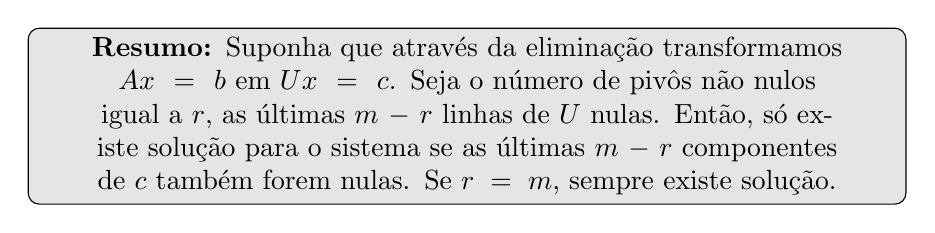
\begin{tikzpicture}
      \node[draw, fill=black!10, rounded corners, text width=0.9\textwidth, align=center] {\textbf{Resumo:} Suponha que através da eliminação transformamos $Ax=b$ em $Ux=c$. Seja o número de pivôs não nulos igual a $r$, as últimas $m-r$ linhas de $U$ nulas. Então, só existe solução para o sistema se as últimas $m-r$ componentes de $c$ também forem nulas. Se $r=m$, sempre existe solução.};
   \end{tikzpicture}
\end{center}

A solução geral é a soma de uma solução particular (com todas as variáveis livres iguais a zero) e de uma solução homogênea (com as $n-r$ variáveis livres como parâmetros independentes). Se $r=n$, não existem variáveis livres e o espaço nulo contém somente o vetor $x=0$.

Existem dois casos extremos:
\begin{itemize}
  \item Se $r=n$, então não existem variáveis livres para $x$. (${\mathcal{N}} = \{ 0\}$)
  \item Se $r=m$, então não existem linhas nulas em $U$. (${\mathcal{I}}m(A) = {\mathbb{R}}^m$)
\end{itemize}

A dimensão do espaço coluna ${\mathcal{I}}m(A)$ é igual ao posto $r$, e uma base de ${\mathcal{I}}m(A)$ é formada pelas $r$ colunas de $A$ que correspondem, em $U$, às colunas contendo pivôs.

Para ver isso com mais clareza, considere um exemplo:
\begin{equation*}
  U = 
  \begin{pmatrix}
      d_1 & *&*&*&*&*\\
      0 & 0 & 0 & d_2 & *&*\\
      0 & 0 & 0 & 0 & 0 & d_3\\
      0&0&0&0&0&0
    \end{pmatrix}.
\end{equation*}
É claro que esta matriz tem três linhas independentes. Afirmamos que existem também apenas 3 colunas independentes, não mais, mostrando que as 3 colunas que contém pivôs são L.I. Suponha que existam $c_1,c_2,c_3$ tais que
\begin{equation*}
  c_1
    \begin{pmatrix}
      d_1\\
      0\\
      0\\
      0
    \end{pmatrix}
    + c_2 
    \begin{pmatrix}
      *\\
      d_2\\
      0\\
      0
    \end{pmatrix}
    + c_3 
    \begin{pmatrix}
      *\\
      *\\
      d_3\\
      0
    \end{pmatrix}
    =
    \begin{pmatrix}
      0\\
      0\\
      0\\
      0
    \end{pmatrix}.
\end{equation*}
Então, como os pivôs são diferentes de zero, é claro que $c_1=c_2=c_3=0$. Portanto, estas colunas são l.i. e formam uma base para o espaço coluna de $A$.

O espaço nulo à esquerda de $A$, que é o espaço nulo de $A^T$, é um subespaço de ${\mathbb{R}}^m$. A dimensão deste espaço é fácil de ser encontrada, já que o número de variáveis básicas mais o número de variáveis livres deve ser igual ao número total de colunas: logo, ${\cal{N}}(A^T)$ tem dimensão $m-r$, já que 
\begin{equation*}
   \text{dim}({\mathcal{I}}m(A)) = \text{dim}({\mathcal{I}}m(A^T)) = r.
\end{equation*}
Vamos ver a importância deste espaço mais à frente.

O espaço linha de $A$ tem a mesma dimensão $r$ do espaço linha de $U$, e eles tem a mesma base pois são o mesmo espaço. Isto ocorre pois as linhas de $U$ são combinações lineares das linhas de $A$, e portanto as operações elementares não alteram o espaço, apenas revelam sua base, que é formada pelas linhas não nulas de $U$.

O espaço nulo de $A$ é o espaço nulo de $U$, pois as soluções que satisfazem $Ax=0$ também satisfazem $Ux=0$. As restrições aos vetores do espaço nulo são dadas pelas linhas não nulas de $U$, e assim o número de linhas nulas de $U$ indica a dimensão do espaço nulo ($n-r$, se tivermos $r$ linhas não nulas). Esta dimensão é às vezes chamada de \emph{nulidade} de $A$.

Resumindo todas estas considerações, chegamos ao seguinte resultado.

\begin{teo}[Fundamental da Álgebra Linear, Parte I]
  Seja $A\in {\mathbb{R}}^{m\times n}$ com $r$ linhas l.i. (ou $r$ colunas l.i.). Então,
  \begin{itemize}
  \item[(i)] ${\mathcal{I}}m(A)$ tem dimensão $r$
  \item[(ii)] ${\mathcal{N}}(A)$ tem dimensão $n-r$
  \item[(iii)] ${\mathcal{I}}m(A^T)$ tem dimensão $r$
  \item[(iv)] ${\mathcal{N}}(A^T)$ tem dimensão $m-r$.
  \end{itemize}
\end{teo}

\section{Existência de Inversas}

Sabemos que se $A$ tem uma inversa à esquerda ($BA=I$) e uma inversa à direita ($AC=I$) então as duas inversas são iguais. Agora, através do posto de uma matriz, podemos decidir se ela tem tais inversas ou não: uma inversa existe somente quando o posto da matriz é o maior possível. Sabemos que o posto satisfaz $r\leq m$ e $r\leq n$. Uma matriz $m\times n$ não pode ter mais do que $m$ linhas l.i. ou $n$ colunas l.i. Queremos mostrar então que, quando $r=n$ existe uma inversa à direita, e que quando $r=m$ existe uma inversa à esquerda. No primeiro caso, $Ax=b$ sempre tem solução; no segundo caso, se a solução existir ela é única. Somente uma matriz quadrada pode ter $r=m=n$, e assim somente uma matriz quadrada pode definir um sistema com solução única e existência garantida.

\begin{center}
   \fbox{$\begin{array}{c c c c} \star & \star & \star & \star\\\star & \star & \star & \star \end{array}$} \fbox{$\begin{array}{c c} \star & \star\\ \star & \star\\ \star & \star \\ \star & \star\end{array}$} = \fbox{$\begin{array}{c c} \star & \star\\ \star & \star\end{array}$}
\end{center}

\begin{itemize}
    \item O sistema $Ax=b$ tem pelo menos uma solução $x$ para cada $b$se e somente se as colunas de $A$ geram ${\mathbb{R}}^m$, ou seja, $r=m$. Neste caso, existe uma inversa à direita $C\in {\mathbb{R}}^{n\times m}$ tal que $AC=I_m$, a matriz identidade de ordem $m$. Isto só é possível se $m\leq n$ (caso contrário, existiriam mais colunas l.i. do que $n$, absurdo).
    \item O sistema $Ax=b$ tem no máximo uma solução $x$ para cada $b$ se e somente se as colunas de $A$ forem linearmente independentes, ou seja, $r=n$. Neste caso, o sistema homogêneo só tem solução trivial e a solução geral será apenas uma solução particular, que é única (não há variáveis livres). Assim, existe uma inversa à esquerda $B \in {\mathbb{R}}^{n\times m}$ tal que $BA=I_n$. Isto só é possível se $m\geq n$.
\end{itemize}

No primeiro caso, uma solução possível é $x=Cb$, já que assim teríamos $Ax=ACb=b$. Mas podem existir outras soluções se existirem outras inversas à direita.

No segundo caso, se a solução para $Ax=b$ existir, ela tem que ser $x=BAx=Bb$. Mas a solução pode não existir.

Existem fórmulas simples para as inversas à direita e à esquerda, se elas existirem:
\begin{equation*}
    B=(A^TA)^{-1}A^T \qquad \mbox{ e } \qquad C = A^T(AA^T)^{-1}.
\end{equation*}
O que pode falhar nestas fórmulas é a existência das inversas de $A^TA$ e de $AA^T$. Vamos mostrar (mais à frente) que estas inversas existem quando o posto de $A$ for $n$ ou $m$, respectivamente. Note também que estas inversas (à direita e à esquerda) não são únicas.

\begin{exemplo}[Strang, p. 97]
  Considere a matriz
  \begin{equation*}
    A =
    \begin{pmatrix}
      4 & 0 & 0\\
      0 & 5 & 0
    \end{pmatrix}.
  \end{equation*}
  Como o posto de $A$ é $2$, nossa análise acima sugere uma inversa à direita $C$. De fato, note que
  \begin{equation*}
    AC =
    \begin{pmatrix}
      4 & 0 & 0\\
      0 & 5 & 0
    \end{pmatrix}
    \begin{pmatrix}
      \sfrac{1}{4} & 0\\
      0 & \sfrac{1}{5}\\
      c_{31} & c_{32}
    \end{pmatrix}
    =
    \begin{pmatrix}
      1 & 0\\
      0 & 1
    \end{pmatrix}.
  \end{equation*}
  De fato, existem infinitas inversas à direita; a última linha de $C$ é totalmente arbitrária. Por outro lado, não existe inversa à esquerda, já que a última coluna de $BA$ será nula para qualquer $B$, o que nos impede de obter a matriz identidade com esse produto.

  Para esse exemplo, se usarmos a fórmula $C=A^T(AA^T)^{-1}$, teremos
  \begin{equation*}
    C =
    \begin{pmatrix}
      4 & 0\\
      0 & 5\\
      0 & 0
    \end{pmatrix}
    \begin{pmatrix}
      \sfrac{1}{16} & 0\\
      0 & \sfrac{1}{25}
    \end{pmatrix}
    =
    \begin{pmatrix}
      \sfrac{1}{4} & 0\\
      0 & \sfrac{1}{5}\\
      0 & 0
    \end{pmatrix}.
  \end{equation*}
  Por outro lado, a transposta de $A$ tem infinitas inversas à esquerda:
  \begin{equation*}
    \begin{pmatrix}
      \sfrac{1}{4} & 0 & b_{13}\\
      0 & \sfrac{1}{5} & b_{23}
    \end{pmatrix}
    \begin{pmatrix}
      4 & 0\\
      0 & 5\\
      0 & 0
    \end{pmatrix}
    = I_{2\times 2}.
  \end{equation*}
\end{exemplo}

Para uma matriz retangular, não é possível termos, ao mesmo tempo, existência e unicidade. Se $m\ne n$, não podemos ter $r=m$ e $r=n$. Para uma matriz quadrada, vale o oposto: não é possível termos existência sem unicidade. Pode-se dizer que, para que uma matriz quadrada $A\in {\mathbb{R}}^{n\times n}$ seja não-singular, cada uma das condições seguintes é necessária e suficiente:
\begin{enumerate}
    \item As colunas de $A$ geram ${\mathbb{R}}^n$, de modo que $Ax=b$ tenha ao menos uma solução para cada $b$.
    \item As colunas são independentes, de modo que $Ax=0 \Rightarrow x=0$.
\end{enumerate}

\section{Transformações lineares in\-ver\-sí\-veis. }

Primeiramente, vamos observar alguns exemplos.

\begin{exemplo*}
A transformação linear definida pela diferenciação de um polinômio de ${\cal{P}}_{n}$ e que resulta em um polinômio em ${\cal{P}}_{n-1}$ tem como núcleo o espaço unidimensional de polinômios constantes: $\frac{da_0}{dx} = 0$. Sua imagem é o espaço $n$ dimensional ${\cal{P}}_{n-1}$. A soma da dimensão do núcleo (1) e do posto ($n$) nos dá a dimensão do espaço original.
\end{exemplo*}

\begin{exemplo*}
A integração de $0$ a $x$, vista como transformação linear de ${\cal{P}}_n$ a ${\cal{P}}_{n+1}$ tem núcleo $\{0\}$. Note que a integração não produz polinômios constantes, e portanto não gera todo o ${\cal{P}}_{n+1}$ (ou seja, sua imagem não é todo o espaço de chegada).
\end{exemplo*}

\begin{exemplo}
  A multiplicação por um polinômio fixo como $2+3x$ é uma transformação linear:
  \begin{equation*}
    Ap = (2+3x)(a_0+\ldots+a_nx^n)=2a_0+\ldots+3a_nx^{n+1}.
  \end{equation*}
  Esta transformação leva ${\cal{P}}_n$ em ${\cal{P}}_{n+1}$, com núcleo contendo apenas $p=0$.
\end{exemplo}

Se quisermos investigar, agora de maneira teórica, como decidir se uma transformação linear possui inversa ou não, precisamos refinar alguns conceitos. 

\begin{defi}
   Seja $T$ uma transformação linear de $E$ em $F$. 
   \begin{itemize}
      \item Se Im$(T)=F$, dizemos que $T$ é \emph{sobrejetora}. 
      \item Se o núcleo de $T$ contiver apenas o vetor nulo, dizemos que esta transformação é \emph{injetora}. Isto é equivalente a dizermos que se $T(u)=T(v)$ então $T(u-v)=0 \Rightarrow u-v=0$. 
   \end{itemize}
\end{defi}

\begin{teo}
   Para que $T:E\to F$ seja inversível, é necessário e suficiente que $T$ seja injetora e sobrejetora.
\end{teo}

\begin{proof}
Primeiramente, observe que $T$ possui inversa à direita $Q:F\to E$ se e somente se pudermos escrever
\begin{equation}
	T(Q(v)) = v, \quad \forall \, v \in F.
\end{equation}
Além disso, $T$ possui inversa à esquerda $S:F\to E$ se e somente se pudermos escrever
\begin{equation}
   S(T(u)) = u, \quad \forall \, u \in E.
\end{equation}
\begin{itemize}
   \item \textbf{Afirmação: $T$ é sobrejetora se e somente se possui inversa à direita.} Se $T$ for sobrejetora, então ${\mathcal{I}}m(T) = F$. Desta forma, todos os vetores de $F$ podem ser escritos como resultado da aplicação de $T$ em algum vetor de $E$. Em particular, se tomamos uma base $\beta \subset F$, podemos escolher vetores $u_i$ em $E$ tais que $T(u_i)=v_i$, para cada $v_i\in \beta\subset F$. Como vimos que para definir uma transformação linear basta definirmos o resultado da sua aplicação em elementos de uma base do domínio, basta escolhermos a transformação $Q$ que a cada $v_i$ associa $u_i$ como inversa à direita de $T$; desta forma, $T(Q(v_i)) = T(u_i) = v_i$ para todo $v_i \in F$. Por outro lado, se $T$ admitir inversa à direita $Q:F\rightarrow E$, então para todo $v\in F$, $T(Q(v)) = v$, ou seja, $v=T(w)$ para todo $v \in F$ (com $w=Q(v)$) e assim $T$ é sobrejetora (a imagem de $T$ é todo o $F$). 
   
   \item \textbf{Afirmação: $T$ é injetora se e somente se possui inversa à esquerda.} Se $T$ é injetora, então ela leva um conjunto de vetores l.i. em um conjunto de vetores l.i.: Sejam $\{ u_1,\ldots,u_n\}\subset E$ l.i. Então, 
   \begin{align*}
      &\alpha_1T(u_1)+\ldots+\alpha_nT(u_n)=0 \\
      &\Leftrightarrow T(\alpha_1u_1+\ldots+\alpha_nu_n)=0
   \end{align*}
   Como $T$ é injetora, $T(u)=0 \Rightarrow u=0$ e assim
   \begin{equation*}
      \alpha_1u_1+\ldots+\alpha_nu_n = 0
   \end{equation*}
   Agora, como o conjunto $\{ u_1,\ldots,u_n\}$ é l.i., isso implica que $\alpha_1=\ldots=\alpha_n = 0$. Logo, $\{T(u_1),\ldots,T(u_n)\}$ formam um conjunto l.i. em $F$.

   Assim, se tomarmos uma base $\{u_i\} \subset E$, podemos definir uma base para $F$ se tomarmos $\{T(u_i),v_i\}$, onde os $v_i$ são acrescentados ao conjunto l.i. $Av_i$ se necessário para completar a base; logo, para definirmos uma inversa à esquerda basta tomarmos $S:F\to E$ tal que $S(T(u_i))=u_i$ e $S(v_i)=0$ para todo $i$.
   
   Finalmente, se $T$ possui inversa à esquerda $S:F\rightarrow E$, então $T(u)=0 \Rightarrow u = S(T(u))=S(0)=0$, ou seja, $T$ é injetora.
\end{itemize}
\end{proof}

Se $T:E\to F$ é inversível, dizemos que ela é uma \emph{bijeção} ou um \emph{isomorfismo} entre $E$ e $F$, e que $E$ e $F$ são isomorfos. Um isomorfismo $T:E\rightarrow F$ transforma uma base de $E$ em uma base de $F$ e se uma transformação linear leva uma base de $E$ numa base de $F$, então ela é um isomorfismo. Desta forma, dois espaços vetoriais de dimensão finita isomorfos tem a mesma dimensão; por outro lado, suponha que $E$ é um espaço vetorial de dimensão $n$. Se fixarmos uma base $\{v_i\} \subset E$, podemos definir $T:{\mathbb{R}}^n \rightarrow E$ tal que se $u=(\alpha_1,\ldots,\alpha_n)\in {\mathbb{R}}^n$, $T(u) = T(\alpha_1,\ldots,\alpha_n)=\alpha_1v_1+\ldots+\alpha_nv_n$. Desta forma, $Ae_1=v_1,\ldots,Ae_n=v_n$, em que os $e_i \in {\mathbb{R}}^n$ são os elementos da base canônica do ${\mathbb{R}}^n$. Portanto, $T$ transforma a base canônica do ${\mathbb{R}}^n$ na base de $E$ e portanto define um isomorfismo entre $E$ e ${\mathbb{R}}^n$: em outras palavras, \emph{todo espaço vetorial de dimensão $n$ é isomorfo a ${\mathbb{R}}^n$.}

\begin{exemplo}
    O espaço ${\cal{P}}_n$ tem dimensão $n+1$ e portanto é isomorfo a ${\mathbb{R}}^{n+1}$. O espaço das matrizes ${\cal{M}}(m\times p)$ é isomorfo a ${\mathbb{R}}^{mp}$.
\end{exemplo}

\subsection{Teorema do núcleo e da imagem de uma transformação linear.}

\begin{teo}[do Núcleo e da Imagem]
    Sejam $E,F$ espaços vetoriais de dimensão finita. Para toda transformação linear $T:E\rightarrow F$ temos que 
    \begin{equation*}
        dim(E) = dim{\mathcal{N}}(T)+dim{\mathcal{I}}m(T).
    \end{equation*}
\end{teo}

\begin{proof}
Vamos mostrar que se $\{T(u_i)\}$ é uma base de ${\mathcal{I}}m(T)$ e $\{v_i\}$ é uma base de ${\cal{N}}(T)$, então $\{ u_i,v_i\}$ é uma base de $E$.

Para isto, considere que se tivermos
\begin{equation}
    \label{eq:base}
    \alpha_1u_1+\ldots+\alpha_pu_p+\beta_1v_1+\ldots+\beta_qv_q=0
\end{equation}
então aplicando $T$ dos dois lados da equação, teríamos que $\alpha_1T(u_1)+\ldots+\alpha_pT(u_p)=0$, já que $v_i \in {\mathcal{N}}(T)$. Mas, como $\{T(u_i)\}$ é uma base de ${\mathcal{I}}m(T)$, estes vetores são l.i., e assim $\alpha_i=0$. Portanto, em \eqref{eq:base} teríamos apenas $\beta_1v_1+\ldots+\beta_qv_q=0$. No entanto, como $\{ v_i\}$ é base de ${\mathcal{N}}(T)$, estes vetores são l.i. e logo $\beta_i=0$. Portanto, $\{ u_i,v_i\}$ são l.i. 

Em seguida, considere um vetor arbitrário $w\in E$. Como $T(w)\in {\mathcal{I}}m(T)$, podemos escrever
\begin{align*}
    T(w) &= \alpha_1T(u_1)+\ldots+\alpha_pT(u_p) \\
    &\Leftrightarrow T(w-(\alpha_1u_1+\ldots+\alpha_pu_p))=0.
\end{align*}
Logo, $w-(\alpha_1u_1+\ldots+\alpha_pu_p) \in {\mathcal{N}}(A)$, e portanto podemos escrever
\begin{equation*}
    w-(\alpha_1u_1+\ldots+\alpha_pu_p) = \beta_1v_1+\ldots+\beta_qv_q,
\end{equation*}
o que implica que $w=\alpha_1u_1+\ldots+\alpha_pu_p+\beta_1v_1+\ldots+\beta_qv_q$, e assim estes vetores geram $E$.
\end{proof}

\begin{coro}
    Sejam $E,F$ espaços vetoriais de mesma dimensão finita $n$. Uma transformação linear $T:E\rightarrow F$ é injetiva se e somente se é sobrejetiva e portanto, é um isomorfismo.
\end{coro}
\begin{proof}
Com efeito, temos 
\begin{equation*}
   n=dim{\mathcal{N}}(T) + dim{\mathcal{I}}m(T).
\end{equation*}
Logo, $dim{\cal{N}}(T)=0 \Leftrightarrow dim{\mathcal{I}}m(T)=n$.
\end{proof}

\begin{exemplo}
   Descrever a imagem e o núcleo de 
   \begin{equation*}
      A = \begin{pmatrix} 1 & -1 \\ 0 & 0\end{pmatrix}
   \end{equation*}
   e
   \begin{equation*}
      B = \begin{pmatrix} 1 & 0 & 1\\ 5 & 4 & 9\\ 2 & 4 & 6\end{pmatrix}
   \end{equation*}
   
   Note que ${\mathcal{I}}m(A) = span\{ (1,0)\}$ e ${\mathcal{N}}(A) = span\{ (x_1,x_1)\} = span\{ (1,1)\}$. A dimensão de cada um dos espaços é 1 e sua soma é 2.

   Para $B$, lembre que ${\mathcal{N}}(B) = {\mathcal{N}}(U)$ (em que $U$ é a matriz obtida depois que escalonamos a matriz $B$) e que ${\mathcal{I}}m(B)$ não é igual a ${\mathcal{I}}m(U)$, mas as colunas que geram a imagem de $B$ são as colunas correspondentes às colunas em que aparecem os pivôs de $U$. Logo, para resolver este problema primeiro escalonamos a matriz $B$. Assim, ${\mathcal{N}}(B) = span\{ (1,1,-1)\} = span\{ (-1,-1,1)\}$ e ${\mathcal{I}}m(B) = span\{ (1,0,0), (0,1,1)\}$. Note ainda que $dim({\mathcal{N}}(B)) + dim({\mathcal{I}}m(B)) = 1+2=3$.   
\end{exemplo}

\begin{exemplo}
   \begin{equation*}
      A = \begin{pmatrix} 1 & 3 & 3 & 2\\2 & 6 & 9 & 5\\-1 & -3 & 3 & 0\end{pmatrix}
   \end{equation*}
\end{exemplo}

\paragraph*{Observação} Toda solução de um sistema $Ax=b$ é soma de uma solução particular (onde todas as variáveis livres valem 0) e de uma solução ao sistema homogêneo $Ax=0$. Isto é equivalente a dizermos que o núcleo e a imagem de $A$ se completam em dimensão para formar o espaço de saída.
\begin{exemplo}
   \begin{equation*}
      Ax = b: \begin{pmatrix} 1 & 2 & 0 & 1\\ 0 & 1 & 1 & 0\\ 1 & 2 & 0 & 1\end{pmatrix}\begin{pmatrix} x_1\\x_2\\x_3\\x_4\end{pmatrix} = \begin{pmatrix} 1\\2\\1\end{pmatrix}
   \end{equation*}
   
   solução geral = solução particular + solução homogênea:

   \begin{equation*}
      x = \begin{pmatrix} 1\\0\\2\\0\end{pmatrix} + x_2 \begin{pmatrix}-2\\1\\-1\\0\end{pmatrix} + x_4\begin{pmatrix} -1\\0\\0\\1\end{pmatrix}
   \end{equation*}
\end{exemplo}

\section{Mudança de base}

Sejam $U=\{u_1,\ldots,u_n\}\subset E$ e $W=\{w_1,\ldots,w_m\}\subset F$ bases em relação às quais a matriz da transformação linear $T:E\rightarrow F$ é definida. Isto significa que para cada $u_j \in U$ definimos a transformação $T$ como sendo $T(u_j) = v_j$, em que $v_j \in F$. Assim, $v_j$ pode ser escrito como combinação linear dos elementos de $W$ (pois $W$ é base de $F$) e assim existem $a_{ij}\in {\mathbb{R}}$ tais que
\begin{equation*}
   T(u_j) = v_j = \sum_{i=1}^m a_{ij}w_i, \qquad (j=1,\ldots,n).
\end{equation*}
Tomando novas bases $U'=\{u_1',\ldots,u_n'\}\subset E$ e $W'=\{w_1',\ldots,w_m'\}\subset F$, a transformação linear $T$ tem uma nova matriz $A'$ definida por
\begin{equation}\label{eq:bases}
  T(u_j') = \sum_{r=1}^m a_{rj}'w_r', \qquad (j=1,\ldots,n).
\end{equation}
Para obtermos a relação entre as matrizes $A$ e $A'$, consideramos as matrizes de mudança de base $P = I^{U'}_U\in {\mathbb{K}}^{n\times n}$ e $Q = I^{W'}_{W}\in {\mathbb{K}}^{m\times m}$ definidas pelas igualdades
\begin{equation*}
  u_j'=\sum_{k=1}^n p_{kj}u_k \qquad \mbox{ e } \qquad w_r'=\sum_{i=1}^m q_{ir}w_i.
\end{equation*}
Agora, podemos escrever cada um dos membros de \eqref{eq:bases} em termos da base $W$, fazendo
\begin{align*}
  T(u_j') = \sum_{k=1}^n p_{kj}T(u_k) &= \sum_{k=1}^n p_{kj}\sum_{i=1}^m a_{ik}w_i\\
  &= \sum_{k=1}^n \sum_{i=1}^m p_{kj}a_{ik} w_i\\
  &= \sum_{i=1}^m \left( \sum_{k=1}^n a_{ik}p_{kj}\right) w_i,
\end{align*}
e
\begin{align*}
  \sum_{r=1}^m a_{rj}'w_r'&=\sum_{r=1}^m a_{rj}' \sum_{i=1}^m q_{ir}w_i\\
  &= \sum_{r=1}^m \sum_{i=1}^m a_{rj}'q_{ir}w_i\\
  &= \sum_{i=1}^m \left( \sum_{r=1}^m q_{ir}a_{rj}' \right) w_i.
\end{align*}
Igualando os coeficientes de $w_i$, temos que
\begin{equation*}
  \sum_{k=1}^n a_{ik}p_{kj} = \sum_{r=1}^m q_{ir}a_{rj}',
\end{equation*}
ou seja, $AP = QA'$.

Observe agora que toda matriz de mudança de base é inversível: leva uma base numa base. Assim, podemos concluir que
\begin{equation*}
  A'=Q^{-1}AP.
\end{equation*}
É útil também observar que se $U$ é uma base de ${\mathbb{R}}^n$, então a matriz de mudança de base da base canônica para $U$ é aquela cujas $n$ colunas são os vetores $u_1,\ldots,u_n$.

No caso particular de um operador $T:E\rightarrow E$ e de suas matrizes $A$ e $A'$ relativas às bases $U$ e $U'$, temos uma única matriz de mudança de base $P$, o que nos dá
\begin{equation*}
  A'=P^{-1}AP.
\end{equation*}

\section{Soma direta}

Como vimos que a imagem e o núcleo de uma transformação linear são complementares com relação à dimensão do espaço vetorial em que estão contidos, podemos imaginar uma decomposição do espaço nestes dois subespaços. 

Vimos anteriormente que se $F_1$ e $F_2$ são subespaços do espaço vetorial $E$, o subespaço vetorial de $E$ formado pela conjunção dos elementos de $F_1$ e de $F_2$  é o conjunto $F_1+F_2$ de todas as somas $u+v$, onde $u\in F_1$ e $v\in F_2$. No caso particular em que $F_1 \cap F_2 = \{ 0\}$, escrevemos $F_1\oplus F_2$ e chamamos esta operação de \emph{soma direta}.

Existe uma noção análoga à de soma direta, que é o produto cartesiano de dois espaços vetoriais $E_1$ e $E_2$. Estes dois espaços não precisam fazer parte do mesmo espaço $E$. Os elementos do conjunto $E_1\times E_2$ são pares ordenados $(u,v), u\in E_1, v\in E_2$. As operações que tornam este novo espaço um espaço vetorial são
\begin{align*}
  &(u,v)+(u',v')=(u+u',v+v'), \\
  &\alpha(u,v)=(\alpha u,\alpha v).
\end{align*}
O vetor nulo é $(0,0)$ e o inverso aditivo é $(-u,-v)$.

Se $\{u_1,\ldots,u_m\} \subset E_1$ e $\{v_1,\ldots,v_k\} \subset E_2$, é imediato observarmos que 
\begin{equation*}
\{(u_1,0),\ldots,(u_m,0),(0,v_1),\ldots,(0,v_k)\}\subset E_1\times E_2
\end{equation*}
é uma base, de modo que $dim(E_1\times E_2) = dim E_i + dim E_2$.

Se $F_1,F_2$ são subespaços de $E$ com $F_1\cap F_2=\{ 0\}$, então a transformação linear
\begin{equation*}
  A:F_1\times F_2 \rightarrow F_1 \oplus F_2
\end{equation*}
definida por $A(u,v) = u+v, u\in F_1, v\in F_2$ é um isomorfismo, pois se 
\begin{equation*}
   \{u_1,\ldots,u_m\}\subset F_1
\end{equation*}
e 
\begin{equation*}
   \{v_1,\ldots,v_n\}\subset F_2
\end{equation*}
são bases, então a base 
\begin{equation*}
   \{(u_1,0),\ldots,(u_m,0),(0,v_1),\ldots,(0,v_n)\}\subset F_1\times F_2
\end{equation*}
é transformada por $A$ no conjunto 
\begin{equation*}
   \{u_1,\ldots,u_m,v_1,\ldots,v_n\}
\end{equation*}
que é, por sua vez, uma base de $F_1\oplus F_2$. Segue-se que $dim(F_1\oplus F_2)=dimF_1+dimF_2=m+n$.

No caso mais geral, em que a interseção $F_1\cap F_2$ não se reduz necessariamente ao vetor nulo, a soma $F_1+F_2$ pode não ser mais uma soma direta, mas ainda podemos definir a transformação linear
\begin{equation*}
  A:F_1\times F_2 \rightarrow F_1+F_2
\end{equation*}
de forma que $A(u,v)=u+v$. Obviamente, $A$ é sobrejetiva: todo elemento de $F_1+F_2$ pode ser representado como imagem por $A$ de um vetor em $F_1\times F_2$. Seu núcleo é formado pelos pares $(u,v)$ tais que $u+v=0$, ou seja $v=-u$. Neste caso, ambos $u,v\in F_1 \cap F_2$. A correspondência $u\mapsto (u,-u)$ é um isomorfismo entre $F_1\cap F_2$ e ${\cal{N}}(A)$. Pelo Teorema do Núcleo e da Imagem, temos então que
\begin{align*}
  dim F_1+dim F_2 &= dim(F_1\times F_2)\\
  &= dim {\cal{N}}(A)+dim(F_1+F_2)\\
  &= dim(F_1\cap F_2) + dim(F_1+F_2).
\end{align*}
Assim, enunciamos o seguinte teorema.
\begin{teo}
  Sejam $F_1, F_2$ subespaços de dimensão finita de um espaço vetorial $E$. Temos que
  \begin{equation*}
    dim F_1+dimF_2 = dim(F_1\cap F_2)+dim(F_1+F_2).
  \end{equation*}
\end{teo}

A noção de soma direta está intimamente ligada à noção de projeção. Se $E=F_1\oplus F_2$ é a decomposição do espaço vetorial $E$ como soma direta destes subespaços, definimos o operador $P:E\rightarrow E$, projeção de $E$ sobre $F_1$ paralelamente a $F_2$ da seguinte maneira: todo vetor $w\in E$ se escreve, de modo único, como soma $w=u+v$ de $u\in F_1,v\in F_2$. Escolha então $Pw=u$. % Figura

O operador linear assim definido tem imagem $F_1$ e núcleo $F_2$. Além disso é fácil ver que $P$ é idempotente (ou seja, $P^2=P$). Vamos mostrar a seguir que todo operador linear idempotente é uma projeção. Note primeiramente que se $P^2=P$, então para todo $w\in {\mathcal{I}}m(P)$, temos que $P(w)=w$ pois $w\in {\mathcal{I}}m(P) \Rightarrow w=P(v) \Rightarrow P(w)=P(P(v))=P(v)=w$.

\begin{teo}
  Seja $P:E\rightarrow E$ um operador linear. Se $P^2=P$, então $E$ é a soma direta do núcleo com a imagem de $P$. Além disso, $P$ é a projeção sobre ${\mathcal{I}}m(P)$ paralelamente a ${\mathcal{N}}(P)$.
\end{teo}

\begin{proof}
Todo $v\in E$ se escreve como soma $v=(v-P(v))+P(v)$, onde $P(v) \in {\mathcal{I}}m(P)$ e, como $P(v-P(v))=P(v)-P(P(v))=P(v)-P(v)=0$, vemos que $v-P(v) \in {\mathcal{N}}(P)$. Portanto, $E={\mathcal{N}}(P)+{\mathcal{I}}m(P)$. Se $w\in {\mathcal{N}}(P)\cap {\mathcal{I}}m(P)$, por um lado temos que $P(w)=0$, e por outro $P(w)=w$; logo, $w=0$. Assim, ${\mathcal{N}}(P)\cap {\mathcal{I}}m(P)=\{0\}$ e temos que $E={\mathcal{I}}m(P) \oplus {\mathcal{N}}(P)$. O resto é óbvio.
\end{proof}

\begin{exemplo}
  Para todo operador linear $T:E\rightarrow E$ num espaço vetorial de dimensão finita vale a relação $dim(E)=dim{\mathcal{N}}(T)+dim{\mathcal{I}}m(T)$, mas não temos sempre que esta soma é direta: por exemplo, se $T:{\mathbb{R}}^2 \rightarrow {\mathbb{R}}^2$ é definido por $T(x,y)=(x-y,x-y)$ então tomando $w=(1,1)$ temos que $w=T(v)$ com $v=(2,1)$ e $T(w)=0$, portanto $w\in {\mathcal{I}}m(T)\cap {\mathcal{N}}(T)$.
\end{exemplo}

\begin{defi}
  Uma \emph{involução} é um operador linear $S:E\rightarrow E$ tal que $S^2=I$, ou seja $S(S(v))=v$ para todo $v\in E$.
\end{defi}

Em outras palavras, uma involução é um operador inversível, igual ao seu próprio inverso. Um exemplo é a reflexão (ortogonal) no plano em torno de uma reta que passa pela origem. Veremos agora que toda involução é a reflexão em torno de um subespaço, paralelamente a outro.

\begin{teo}
  Seja $S:E\rightarrow E$ uma involução. Os conjuntos $F_1=\{u\in E: S(u)=u\}$ e $F_2=\{v\in E:S(v)=-v\}$ são subespaços vetoriais e $E=F_1\oplus F_2$. Para todo $w=u+v$ com $u\in F_1, v\in F_2$ tem-se $S(w)=u-v$. Além disso, $P=\frac{1}{2}(S+I)$ é a projeção sobre $F_1$ paralelamente a $F_2$.
\end{teo}

\begin{proof}
Para todo $w\in E$, podemos escrever $w=u+v$, onde $u=\frac{(w+S(w))}{2}$ e $v=\frac{(w-S(w))}{2}$. Como $S^2=I$, é claro que $S(u)=u$ e $S(v)=-v$, ou seja, $u\in F_1, v\in F_2$. É claro também que $F_1\cap F_2=\{0\}$, e que $w=u+v \Rightarrow S(w)=u-v$ se $u\in F_1$ e $v\in F_2$. Finalmente, 
\begin{align*}
   P=\frac{1}{2}(S+I)\Rightarrow P^2 &= \frac{1}{4}(S^2+2S+I)\\
   &= \frac{1}{4}(2S+2I)\\
   &= \frac{1}{2}(S+I)=P.
\end{align*}
Pode-se ver facilmente que o núcleo de $P$ é $F_2$ e a imagem de $P$ é $F_1$.
\end{proof}

O caso mais comum de reflexão é aquele em que se tem $dim(E)=n$, $dim(F_1)=n-1$ e $dim(F_2)=1$, de modo que $S$ é a reflexão em torno do hiperplano $F_1$ paralelamente à reta $F_2$.
